\documentclass[twoside]{article}
\usepackage[a6paper, margin=0.5in]{geometry}
\usepackage{graphicx}
\usepackage{float}
\usepackage{hyperref}
\usepackage{pifont}
\usepackage{titlesec}
\usepackage{enumitem}
\usepackage{fancyhdr}
\usepackage{xcolor}

\pagestyle{fancy}
\fancyhead[L]{User Manual}
\fancyhead[R]{\thepage}
\renewcommand{\headrulewidth}{0.4pt}

\titleformat{\section}{\small\bfseries}{\thesection.}{0.4em}{}
\titleformat{\subsection}{\small\bfseries}{\thesubsection.}{0.4em}{}
\setcounter{tocdepth}{1}

\usepackage{tikz}
\usepackage{adjustbox}

\newcommand{\prevtrack}{%
\adjustbox{valign=c}{%

\begin{tikzpicture}[scale=0.02]
  \filldraw[black] (6,0) -- (6,10) -- (0,5) -- cycle; % Triangle
  \filldraw[black] (12,0) -- (12,10) -- (6,5) -- cycle; % Triangle
  \draw[black, thick] (0,0) -- (0,10); % Bar
\end{tikzpicture}}%
}

\newcommand{\nexttrack}{%
\adjustbox{valign=c}{%

\begin{tikzpicture}[scale=0.02]
  \filldraw[black] (0,0) -- (0,10) -- (6,5) -- cycle; % Triangle
  \filldraw[black] (6,0) -- (6,10) -- (12,5) -- cycle; % Triangle
  \draw[black, thick] (12,0) -- (12,10); % Bar
\end{tikzpicture}}%
}

\newcommand{\downleftarrow}{
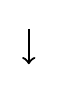
\begin{tikzpicture}[scale=0.15]
  \draw[->, thick] (0,1) -- (0,-1) -- (0,-2);
\end{tikzpicture}
}

\begin{document}
\begin{titlepage}
    \centering
    \vspace*{3cm}
    
    {\Huge \bfseries User Manual \par}
    \vspace{2cm}
    
    \newpage
    Intentionally left blank
    \thispagestyle{empty}
    \newpage
    
    {\Large \bfseries Micro ECG\par}
    \vspace{1cm}
    
    {\Large Developed By\par}
    
    \begin{center}
        \begin{itemize}[leftmargin=3cm]
              \item Raju Adhikary
              \item Tanima Ghosh
              \item Sudipta Sem
              \item Ruma Mandi
              \item Goutam Ambali
        \end{itemize}
    \end{center}
    
    \vfill
    
    {\Large Under Guidance Of\par}
    {\large Souvik Bag(Lec. EE at Ranaghat Government Polytechnic)\par}
    \vfill
    
    {\small Author\par}
    {\small Raju Adhikary\par}
    {\small \today\par}
\end{titlepage}



\vspace{-2em}

\newpage
Intentionally left blank
\thispagestyle{empty}
\newpage

\tableofcontents

\newpage

\section{Overview}
A portable ECG monitor with real-time signal display via wifi and your browser.
\begin{figure}[H]
    \centering
    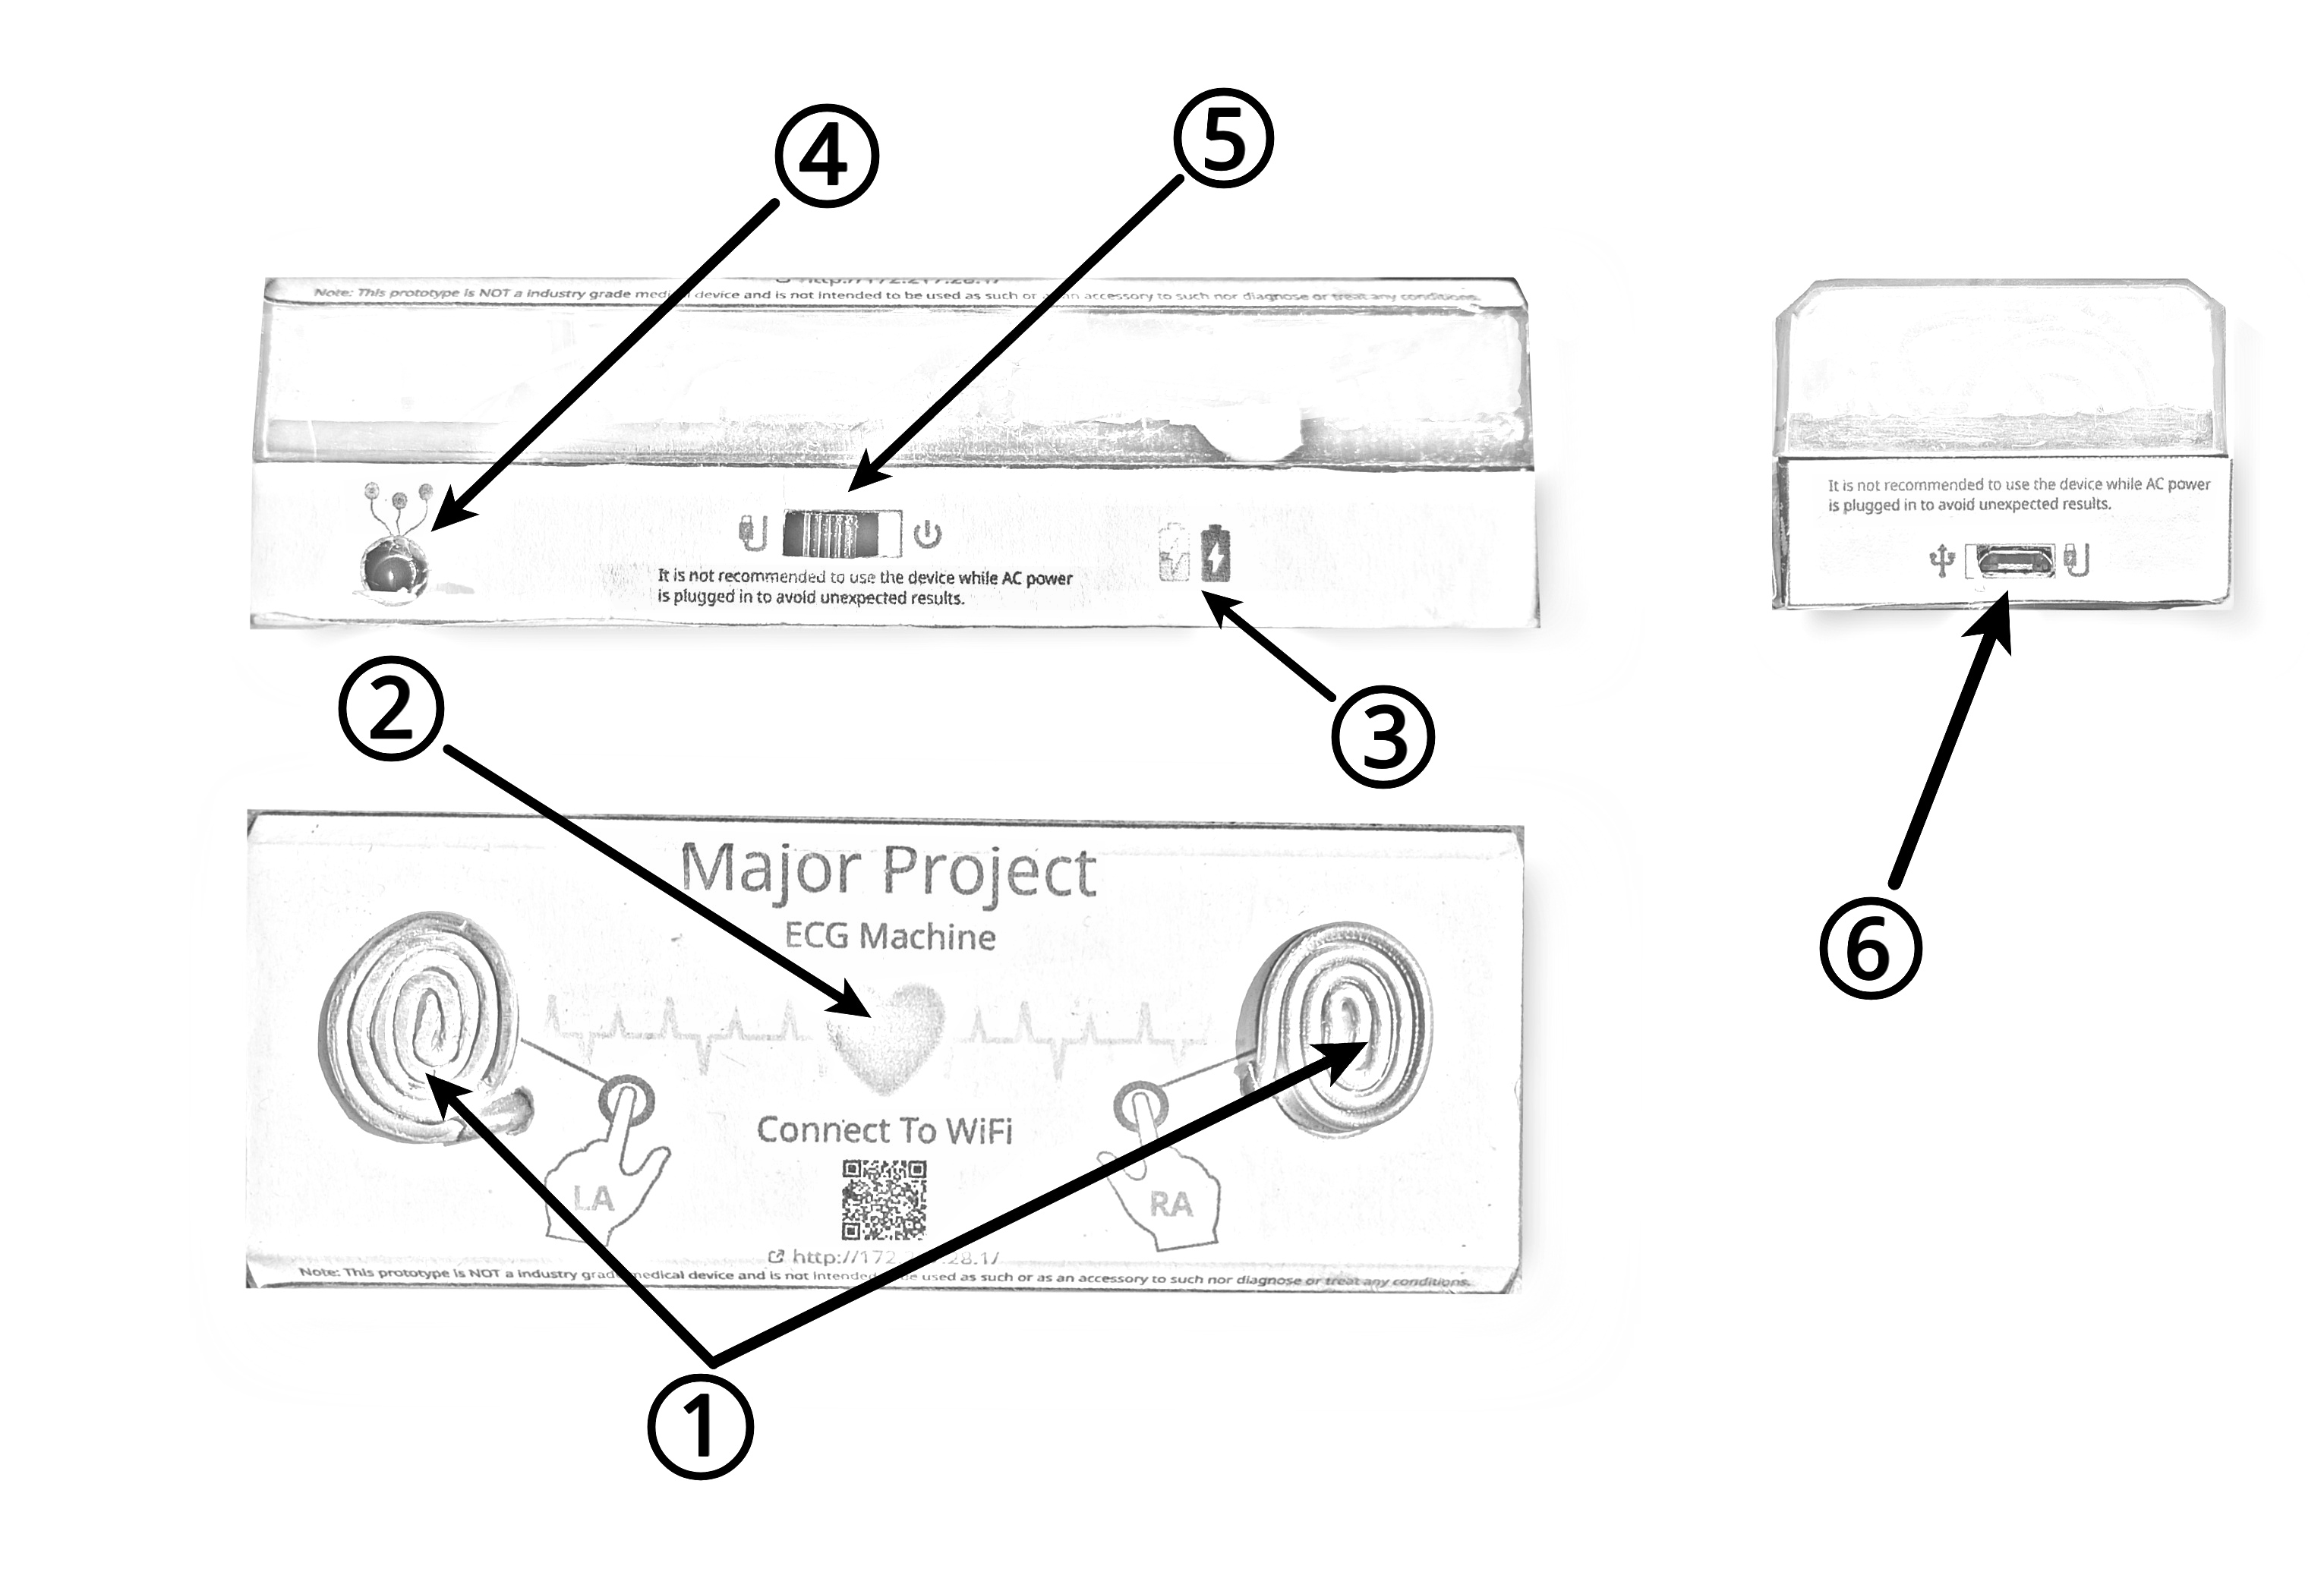
\includegraphics[scale=1.5]{images/prototype-overview.png}
    \caption{Prototype Overview}
    \label{fig:prototype_overview}
\end{figure}
{\small
\begin{enumerate}
    \item \textbf{LA \& RA Electrodes (Touch Type):} Finger placement electrodes for Left Arm (LA) and Right Arm (RA) detection. These are the primary contact points for quick ECG readings.
    \item \textbf{Heart LED Indicator:} Blinks in sync with the detected heart rhythm. Also shows device power status.
    \item \textbf{Charging Status LED:} \textcolor{red}{Red} – Charging,\\ \textcolor{blue}{Blue} – Fully charged.
    \item \textbf{External Electrode Port:} Alternative electrode input, typically for chest placement using gel electrodes for improved accuracy.
    \item \textbf{Slide Switch (Charge-Off-On):} \textit{Charge} – Enables charging without powering on the device.\\ \textit{Off} – Completely powered off.\\ \textit{On} – Powers the device for use.
    \item \textbf{Micro-USB Port:} Used for charging and firmware updates only. \textbf{Note:} Do not use the device while charging to avoid inaccurate results.
\end{enumerate}
}

\section{Specs}
\begin{itemize}[leftmargin=*]
  \item IC: AD8232 (Instrumentation Amp)
  \item MCU: ESP8266 (Wi-Fi 802.11 b/g/n, 2.4 GHz)
  \item ADC: 10-bit @ 300 SPS (Default)
  \item Electrodes: 2x finger (RA, LA), 1x external port (chest)
  \item Filtering: RC + Op-Amp (hardware-side)
  \item Communication: Wi-Fi + WebSocket (live ECG stream)
  \item Battery: 1200mAh (3.7V Li-ion)
  \item Regulator: RT9080 (3.3V LDO)
  \item BMS: TP4056
  \item USB: Micro-USB (charge/update)
  \item Power Switch: 3-position (Charge–Off–On)
  \item LEDs: \textcolor{red}{Heartbeat} (red), \textcolor{red}{Charging} (red), \textcolor{blue}{Full} (blue)
\end{itemize}


\section{Getting Started}
\subsection{Power On}
Slide \textbf{POWER} switch to ON. The heart LED should start blinking.
(If it doesn't blink, ensure the device is charged.)
\subsection{Connect to Wi-Fi}
On your mobile or computer, connect to the device’s Wi-Fi hotspot.
(Note: Only supports 2.4GHz networks.)
\subsection{Open the User Interface}
Once connected to the ECG device's Wi-Fi, a screen should automatically pop up with the web interface. \\
If it doesn’t open by itself, just open any browser (Chrome recommended) and go to: \\
http://172.217.28.1 \\
Chrome tested on mobile, desktop, and laptop — works on cross-platform.
\subsection{ECG Display}
The graph may initially show random noise if electrodes are open.

\subsection{Electrodes}
\begin{itemize}[leftmargin=*]
  \item \textbf{Finger:} Touch LA \& RA on top of the device. OR,
  \item \textbf{Chest:} Connect external electrode (Front-Left side)
\end{itemize}

\subsection{Take Reading}
Once the waveform is stable , no noise on the screen, hold still and observe the heart rate.

\section{Parameters}
\begin{itemize}[leftmargin=*]
    \item \textbf{Heart Rate (BPM):} -  Beats per minute calculated in real-time.
    \item \textbf{QRS Duration:} -  Time interval of the QRS complex, indicating ventricular depolarization.
    \item \textbf{QT Interval:} -  Total time for ventricular depolarization and repolarization.
    \item \textbf{PR Interval:} -  Time from the start of the P wave to the start of the QRS complex.
    \item \textbf{ST Interval:} -  Segment between the end of the S wave and the beginning of the T wave.
\end{itemize}

\section{AI Assistant}
\begin{itemize}[leftmargin=*]
    \item \textbf{Function:} -  ECG data send to a third-party AI for anomaly detection.
    \item \textbf{How to Use:} -  Click on the "Get Assistance" button to initiate the AI analysis.
\end{itemize}

\section{Controls}
\begin{itemize}[leftmargin=*]
    \item \textbf{HOLD:} -  Pauses the real-time ECG display.​
    \item \textbf{RECORD:} -  Starts recording the ECG data.​
    \item \textbf{CLEAR:} -  Clears the current ECG graph from the display.​
    \item \textbf{SNAP:} -  Captures a snapshot of the current ECG graph.​
    \item \textbf{TIME/DIV (-/+):} -  Adjusts the time scale of the ECG graph.​
    \item \textbf{VOLT/DIV (-/+):} -  Adjusts the voltage scale of the ECG graph.
    \item \textbf{POSITION VERTICAL (\ding{115}/\ding{116}):} -  Moves the ECG graph up or down.​
    \item \textbf{POSITION HORIZONTAL (\prevtrack/\nexttrack):} -  Moves the ECG graph left or right.​
\end{itemize}

\section{Recordings}
\begin{itemize}[leftmargin=*]
    \item \textbf{IMPORT (.json):} -  Allows importing of ECG data in JSON format.
    
    \item \textbf{Accessing Recordings:} -  Recorded ECG sessions are listed with timestamps in the RECORDINGS section..​
    \item \textbf{Downloading Recordings:} -  Click on the download (\downleftarrow) icon next to a recording to download the data..​
    \item \textbf{Deleting Recordings:} -  Click on the ($\times$) icon next to a recording to delete it.
\end{itemize}

\section{Settings (Not available - Planned)}
% \begin{itemize}[leftmargin=*]
%   \item WiFi SSID change
%   \item Adjust SPS
%   \item Factory Reset
%   \item Firmware update access
% \end{itemize}

\section{Troubleshooting}
\begin{itemize}
    \item \textbf{No Heart LED Blinking:} \\
    Ensure the device is charged. Slide the power switch OFF and ON again.

    \item \textbf{Cannot Connect to Wi-Fi:} \\
    Confirm your device supports 2.4GHz Wi-Fi. Restart the ECG device and try again.

    \item \textbf{Web Interface Doesn’t Open Automatically:} \\
    Check sign-in notification | open a browser manually (Chrome recommended) and enter\\ \texttt{http://172.217.28.1}.

    \item \textbf{Weak signal:} \\
    Possible Cause: Dry skin, poor contact | Moisten fingers slightly or use external electrode.

    \item \textbf{Data delay in UI:} \\
    Improve WiFi signal, Move closer to the device.

    \item \textbf{ECG Graph Shows Noise:} \\
    Ensure stable positioning, avoid movement. \\
    Make sure the electrodes are placed correctly. Wait a few seconds for the signal to stabilize. \\
    For finger electrodes, gently rub and clean the metal surface before use to improve contact. \\
    \textbf{Do not} try to rub or clean the disposable adhesive external electrodes, as this may damage them.
\end{itemize}

\section{Safety \& Maintenance}
\begin{itemize}[leftmargin=*]
  \item Keep electrodes clean and dry for optimal signal quality.
  \item Use BIS certified charger to charge via Micro-USB.
  \item Do not submerge in water or expose to excessive moisture.
  \item Don't drop or shake.
  \item Update firmware from authorised source only.
  \item Avoid applying excessive force on the device or electrodes.
\end{itemize}
\newpage
Intentionally left blank
\thispagestyle{empty}
\newpage
\section{DISCLAIMER}
    This project prototype is intended solely for \textbf{educational, research, prototyping, and demonstration purposes}. It is \textbf{not designed, tested, certified, or approved} for any form of \textbf{medical, clinical, diagnostic, or therapeutic use}.

    This prototype must \textbf{not be used in life-critical systems}, \textbf{healthcare settings}, or for \textbf{monitoring or treating humans or animals}. It has \textbf{not been reviewed or approved} by any medical or regulatory authority, including but not limited to the \textbf{Central Drugs Standard Control Organisation (CDSCO)} or similar bodies.

    The developers of this project make \textbf{no representations or warranties} of any kind, express or implied, regarding its \textbf{accuracy, safety, reliability, or suitability} for any purpose beyond learning and experimentation.

    By using this prototype, the user assumes \textbf{full responsibility and liability} for its use and agrees that it is provided \textbf{“as is”}, without any warranty of any kind, including but not limited to warranties of \textbf{merchantability}, \textbf{fitness for a particular purpose}, or \textbf{non-infringement}.

    Use of this prototype implies full \textbf{understanding and acceptance} of this disclaimer.
\newpage
:)
\thispagestyle{empty}
\end{document}